\subsection{A certified interval for the transition}
\label{sec:enclosure}

\begin{proposition}\label{prop:enclosure}
The critical Gaussian smoothing time modulo four satisfies
\[
                   0.04007656562<h_*<0.04007656609 .
\]
The interval has width $4.7\times10^{-10}$. In particular both classes lead with positive logarithmic density at
$h=0.04$.
\end{proposition}

\begin{proof}
The external numerical input consists of the first ten consecutive
positive ordinates of $\beta$, counted with multiplicity, and the fact
that the eleventh exceeds $32$. The LMFDB record for the primitive
character $4.3$ supplies the ordinates. Its reliability page specifies
interval-arithmetic accuracy to one unit in the last displayed place
and completeness through the range shown. The first and tenth
ordinates are approximately $6.0209489047$ and $29.6563840146$; the
eleventh is approximately $32.5921865271$. The certificate truncates
the ten entries to $22$ places after the decimal point and allows
error $10^{-21}$ at each center.%
\footnote{The LMFDB, \emph{Dirichlet $L$-function $1$-$2$e$2$-$4.3$-r$1$-$0$-$0$},
\url{https://www.lmfdb.org/L/1/2e2/4.3/r1/0/0}.
The linked Reliability and Source pages give the error and completeness
statements and attribute the computation to David Platt.}

For a short independent tail estimate, let $D$ denote the completed
logarithmic derivative from the preceding subsection. Its paired
Hadamard formula gives
\[
 \sum_{\gamma>0}\frac{m_\gamma}{9/4+\gamma^2}
   =\frac{D(2)}{3}<1.
\]
Indeed
$D(2)=\tfrac12\log(4/\pi)+\tfrac12\psi(3/2)+\beta'(2)/\beta(2)$,
where $\psi$ is the digamma function. The first two terms together
are less than one, since $\psi(3/2)<\psi(2)=1-\gamma_{\rm E}<1$.
The Euler series bounds the last term in absolute value by
$\sum_{n\ge2}(\log n)n^{-2}<2$, by comparison with its integral.
For either endpoint $h$ in the proposition, $(9/4+u^2)e^{-hu^2}$
decreases for $u\ge32$. Thus the absolute contribution of all
omitted harmonics is at most $2(9/4+32^2)e^{-h32^2}<4\cdot10^{-15}$.

Write $h_-=0.04007656562$, $h_+=0.04007656609$ and
$t_0=59260005815.44527175543962534$, all taken as exact rationals.
At $h_-$ the time $t_0$ supplies one admissible point of the compact
phase group. At $h_+$ the triangle inequality bounds every phase at
once. The complete enclosures, including the tail, are
\begin{align*}
 -2445384\cdot10^{-15}
 &\le \tfrac12+2\sum_{\gamma>0}m_\gamma
      e^{-h_-\gamma^2}\cos(\gamma t_0)
    \le-74977\cdot10^{-15},\\
 47190\cdot10^{-15}
 &\le \tfrac12-2\sum_{\gamma>0}m_\gamma e^{-h_+\gamma^2}
    \le47197\cdot10^{-15}.
\end{align*}
The first upper bound is negative and the second lower bound is
positive. Strict monotonicity of the minimum proves the claim.

The file \texttt{certify\_threshold.py} reproduces these inequalities
using integer and rational arithmetic. It encloses $\pi$ by
Machin's formula, reduces each cosine argument, and bounds the
Taylor remainders for the exponential and cosine. Moving any one
input ordinate within its radius $\varepsilon$ changes a doubled
summand by at most $2(64h+|t_0|)\varepsilon$; for the amplitude
bound one can set $t_0=0$ in this estimate. This accounts for
the amplification of ordinate errors at the large witness time.
\end{proof}

\begin{figure}[htb]
\centering
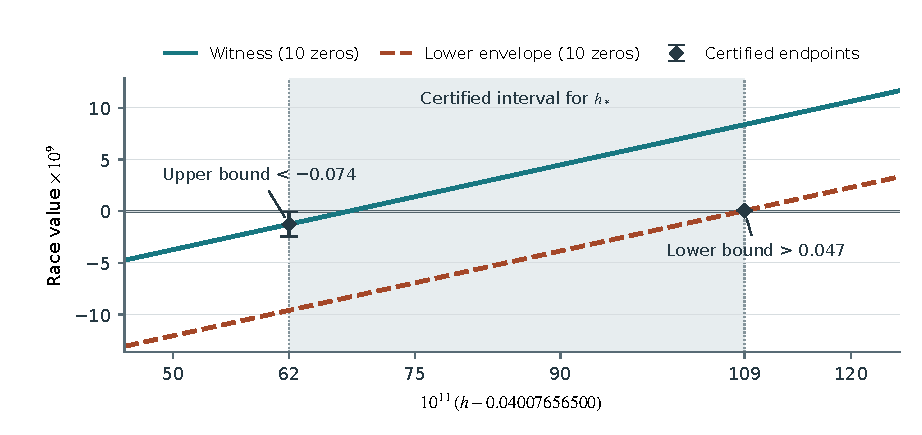
\includegraphics[width=.88\linewidth]{threshold_bounds.pdf}
\caption{Two bounds on the limiting minimum near its zero. The upper curve evaluates one time shared by all ten retained harmonics. The lower curve gives each harmonic its most negative possible value. The plotted curves use the ten-term sums. Diamonds mark the midpoints of the certified endpoint enclosures. The vertical bars include ordinate uncertainty and the full spectral tail. The bar at the right endpoint is smaller than its marker. Opposite strict signs certify the shaded interval.}
\end{figure}
